À partir de ces différentes contraintes définies précédemment, celles sur les noyaux $w$ et celles sur les paramètres de contrôle $\alpha$ des couches morphologiques, on crée finalement une \textit{loss} personnalisable, dans laquelle on ajoute les contraintes que l'on souhaite, chacune pondérée par un hyperparamètre propre à elle-même. C'est à l'utilisateur de choisir les contraintes à intégrer selon les contextes, selon la géométrie visée des noyaux du réseau, et selon les valeurs des $\alpha$ recherchées. Cependant, plus il y a de contraintes différentes ajoutées dans la fonction de perte \textit{loss}, plus le réseau aura tendance à << délaisser >> certaines contraintes pour d'autres, lors de son entraînement, et moins le réseau convergera bien et sera performant à la fin. \\

\vspace{-1.6mm}
\noindent Dans notre cas, les huit fonctions structurantes cibles étudiées ayant des propriétés géométriques bien différentes, l'application d'une même contrainte géométrique parmi celles développées n'est pas adaptée. On peut cependant, dans le cadre des échecs de la partie précédente sur les réseaux à deux couches, faire l'hypothèse forte (que l'on n'utilisera pas dans des contextes où l'on ignore l'hypothèse) que l'on veut que les réseaux se comportent soit comme une ouverture, soit comme une fermeture. On prend ainsi la seconde contrainte sur les paramètres de contrôle $\alpha$, l'erreur sur l'éloignement opposé (formule \ref{erreur_awayOPP}), qu'on applique sur l'ensemble des expériences de la partie précédente, avec toujours un partage de poids doux en plus. \\

\vspace{-1.6mm}
En reprennant la même méthodologie que dans les parties précédentes avec des réseaux $\mathcal{S}$MorphNetTanh à deux couches, on obtient, pour l'opération cible d'ouverture et la banque d'images d'entraînement MNIST, les résultats suivants (fig. \ref{fig:MSEpFSIMvsMSEpFSIMpASIM_opening}) : \\

% figure
\vspace{1.0mm}
\begin{figure}[!htp]
  \begin{center}
  
    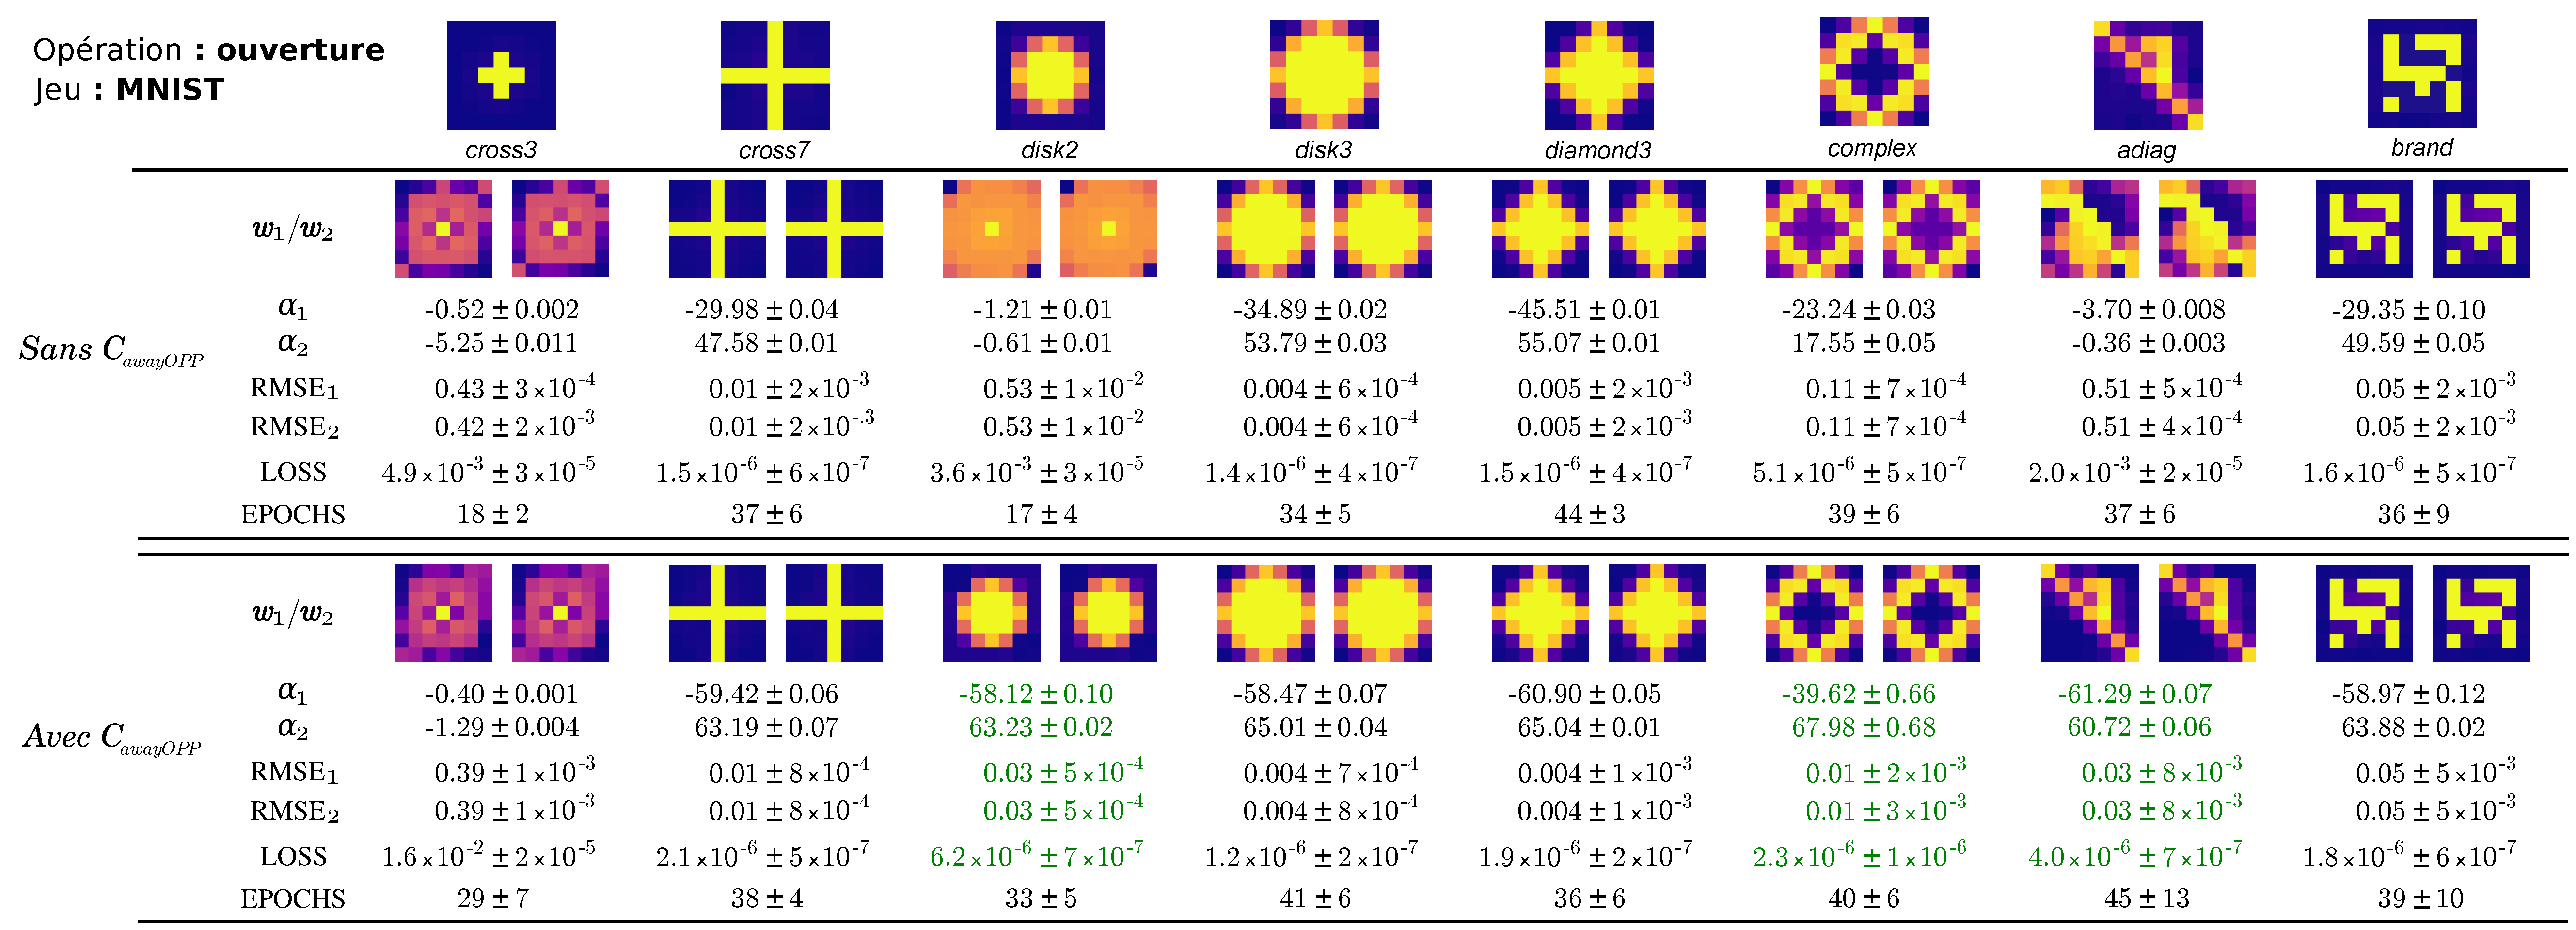
\includegraphics[width=1.00\linewidth]{parts/3-contributions/C-contraintes_geometriques/figures/f_opening_mnist.pdf}
    \vspace{-4.0mm}
    \caption{ \centering Comparaison des poids appris et des moyennes et écarts-types des métriques $\alpha$, \textit{RMSE}, \textit{loss} et nombre d'époques, et ce sur six runs, entre sans et avec la contrainte $C_\text{awayOPP}$, pour les huit fonctions structurantes cibles et l'opération d'\textbf{ouverture}.}
    \label{fig:MSEpFSIMvsMSEpFSIMpASIM_opening}
    
  \end{center}
\end{figure}


\newpage

On obtient également, pour l'opération cible de fermeture et la banque MNIST avec des réseaux $\mathcal{S}$MorphNetTanh à deux couches, les résultats suivants (fig. \ref{fig:MSEpFSIMvsMSEpFSIMpASIM_closing}) : \\

% figure
\vspace{1.6mm}
\begin{figure}[!htp]
  \begin{center}
  
    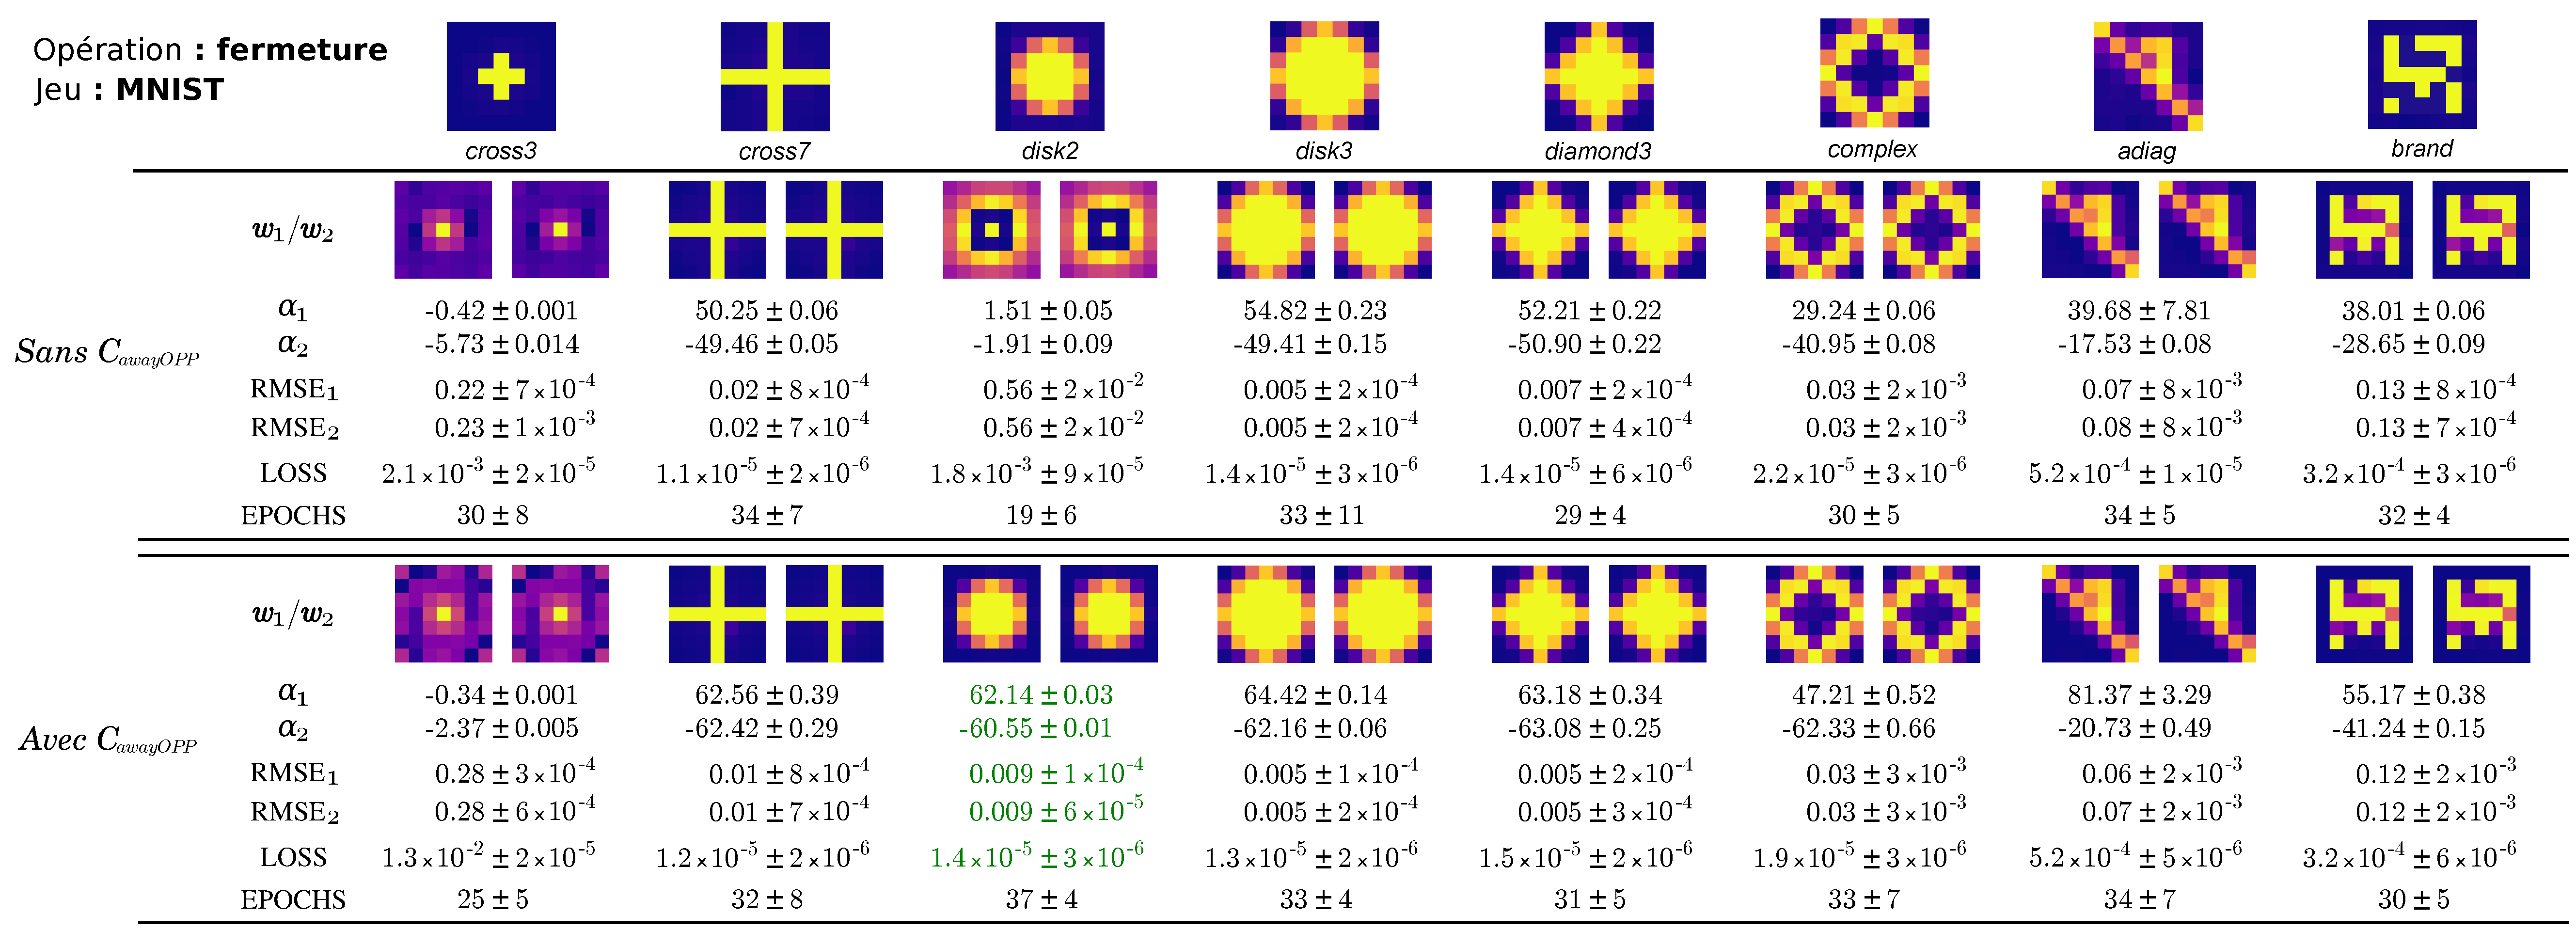
\includegraphics[width=1.00\linewidth]{parts/3-contributions/C-contraintes_geometriques/figures/f_closing_mnist.pdf}
    \vspace{-4.0mm}
    \caption{ \centering Comparaison des poids appris et des moyennes et écarts-types des métriques $\alpha$, \textit{RMSE}, \textit{loss} et nombre d'époques, et ce sur six runs, entre sans et avec la contrainte $C_\text{awayOPP}$, pour les huit fonctions structurantes cibles et l'opération de \textbf{fermeture}.}
    \label{fig:MSEpFSIMvsMSEpFSIMpASIM_closing}
    
  \end{center}
\end{figure}


\vspace{-1.0mm}
Les résultats de convergence de $\mathcal{S}$MorphNetTanh sur les figures \ref{fig:MSEpFSIMvsMSEpFSIMpASIM_opening} et \ref{fig:MSEpFSIMvsMSEpFSIMpASIM_closing}, montrant l'état final des noyaux des réseaux et les valeurs des métriques de performances associées pour les différentes expériences réalisées, permettent de mettre en évidence l'efficacité de la métrique de contrainte $C_\text{awayOPP}$, qui influe sur les paramètres de contrôle $\alpha$, et qui est ici associée à un partage de poids doux, dans le cadre d'une opération cible d'ouverture (\ref{fig:MSEpFSIMvsMSEpFSIMpASIM_opening}) et de fermeture (\ref{fig:MSEpFSIMvsMSEpFSIMpASIM_closing}) sur des réseaux à deux couches. \\

\vspace{-0.6mm}
\noindent Les résultats en couleur verte sont ceux pour lesquels les réseaux avec cette contrainte $C_\text{awayOPP}$ ont de bien meilleurs résultats. Cela concerne en particulier les expériences avec \textit{disk2}, \textit{complex} et \textit{adiag} pour l'ouverture, et l'expérience avec \textit{disk2} pour la fermeture. On obtient les mêmes résultats avec les expériences faites sur FashionMNIST. Pour ces expériences-là, la contrainte $C_\text{awayOPP}$ couplée à un partage de poids doux a permis au réseau de bien converger vers l'état cible, avec une forme des noyaux proche de celle de la fonction structurante cible, et avec des valeurs de $\alpha$ du bon signe et éloignées de $0$ (on a donc plus une opération exacte qu'une pseudo-opération). \\

\vspace{-0.6mm}
\noindent Cependant, on remarque qu'il existe toujours une fonctions structurante cible pour laquelle cette contrainte n'a pas d'impact, et ce à la fois pour l'ouverture et la fermeture : \textit{cross3}. En examinant les valeurs de $\alpha$, on remarque qu'elles restent très proches de $0$ et sont du même signe, malgré la présence de la contrainte $C_\text{awayOPP}$. Elle n'est donc pas encore suffisante pour améliorer la convergence de l'ensemble des échecs.
